%

\subsection{Sous-Activit\'{e}} \label{act12}
\paragraph{But de la sous-activit\'{e}}
Produire la classe  traitant \ldots
\paragraph{Description}
Description de la sous-activit\'{e} 1.2, \`{a} d\'{e}crire.

\begin{enumerate}
    \item sous-sous-activit\'{e} \`{a} d\'{e}crire.
    \begin{enumerate}
    \item sous-sous-sous-activit\'{e} \`{a} d\'{e}crire.
    \end{enumerate}
\end{enumerate}

\section{Ajout de jReplay} \label{act2}
\subsection*{But de l'activit\'{e}}
jReplay doit servir � garder la trace de l'activit� d'un
utilisateur afin de faire ex�cuter le programme par un d�veloppeur
qui doit trouver le probl�me conduisant � un bug.


\subsection*{Description}
Description de l'activit\'{e} 1, \`{a} d\'{e}crire.

\begin{itemize}
\item Faire un analyse des possibles solutionnes

\item Analyser las solutions avec le pattern observer

\item Analyser la compatibilit� avec la solution actuelle

\item Trouver les �quivalences

\item D�finir un diagramme UML de l'implementation du pattern
observer avec les menus \ref{observer}.


\item D�finir un diagramme UML de l'implementation du pattern
observer avec les dialogs.

\item D�finir un diagramme UML de l'implementation du pattern
observer avec la TTStructure.

\item D�finir un diagramme UML de l'implementation du pattern
observer avec la State Bar.

\item D�finir un diagramme UML de l'implementation du pattern
observer avec la ToolBar.

\item Menus � revoir  aire dans le menu Fichier
    \begin{itemize}
    \item Horaire cycle \pro{NewTTSCyCmd} (Non Fait)
    \item Horaire examen \pro{NewTTSExCmd} (Non Fait)
    \item Grille cycle
    \item Grille examen
    \item Ouvrir horaire \pro{OpenTTDlg} (Fait) \pro{changeInDModel()} � v�rifier
    \item Ouvrir grille \pro{OpenTTSDlg} \pro{DMediator.addDoc} \pro{Dmodel constructeur}  (Fait)
    \item Enregistrer
    \item Enregistrer sous
    \item D�finir fichiers � importer \pro{DefFilesToImportDlg} Rien
    \item Importer automatiquement
    \item Exporter
    \end{itemize}

\item Changements � faire dans le menu Affectation
    \begin{itemize}
    \item Activit�s \pro{ActivityDlg} \pro{changeInDModelByBuildMatrixConflicts}
    (Fait) \\
    Double click Activiti�s \pro{EditActivityDlg} \pro{changeInDModelByEditActivityDlg} (Fait)
    \item Groupes
    \item Enseignants \pro{InstructorAvailabiliyDlg} \pro{changeInDModelByInstructorsDlg} (Fait)
    \item Locaux \pro{RoomsAvailabilityDlg} \pro{changeInDModelByRoomsDlg}(Fait)
    \item �v�nements \pro{EventsDlg}
    \pro{changeInDModelByEventsDlg}(Fait)
    Double click �v�nements \pro{EditActivityDlg} \pro{changeInDModelByEditActivityDlg} (Fait)
    \item D�finir ensemble Rien
    \item Grille partielle Rien
    \item Affectation manuelle Modifie \pro{EditActivityDlg} \pro{changeInDModelByEditActivityDlg} (Fait)
    \end{itemize}

\item Changements � faire dans le menu Modification
    \begin{itemize}
    \item Activit�  Dlouble click \pro{ActivityModifDlg} \pro{ChangeInDModelByModifyRemove} \\
    \pro{ChangeInDModelByModifyAdd}(Fait) � v�rifier
    \end{itemize}

\item Changements � faire dans le menu Optimisation
    \begin{itemize}
    \item Affectation Initiale \pro{InitialAssignCmd}
    \pro{changeInDModel()}(Fait)
    \item Construire l'horaire
    \item Formation de groupes Balanc� Rien
    \item Formation de groupes Interm�diaire Rien
    \item Formation de groupes Optimise Rien
    \end{itemize}
\item Changements � faire dans le menu Preferences
    \begin{itemize}
    \item Option L\& F Rien
    \item Options conflits !!ATTENTION!! \pro{Prefereces} \pro{ConflictDlg}
    \item Affichage grille Simple, D�taille Split H et D�taille
    Rien
    Split V

    \end{itemize}
\item Changements � faire dans le menu Aide
    \begin{itemize}
    \item About Rien
    \end{itemize}

\item Changements � faire dans le menu Beta Test
    \begin{itemize}
    \item Formation des groupes personnalis�e
    \item Importation S�lective Enseignants
    \item Importation S�lective Locaux
    \item Importation S�lective Activit�s
    \item Importation S�lective �tudiants
    \end{itemize}


\item Changements � faire dans le menu D�veloppement
    \begin{itemize}
    \item fichier1.dia \pro{MyFileCmd} \pro{changeInDModel()}
    \end{itemize}
\end {itemize}

\begin{figure}[ht]
\begin{center}
%\includegraphics[width=4in]{activities/mouseTrap/observer.eps}
\mbox{\epsfysize 4.0in
\epsfbox{activities/mouseTrap/observer.eps}} \caption{Pattern
Observer dans Diamant} \label{observer}
 \end{center}


\end{figure}



\subsection{Validation du prototype} \label{act21}
\paragraph{But de la sous-activit\'{e}}
� venir.
\paragraph{Description}
� venir.

\subsection{Modification du code} \label{act22}
\paragraph{But de la sous-activit\'{e}}
� venir.
\paragraph{Description}
� venir.
